\chapter{Summary}
Das Projekt BestShift wird wie folgt durchgeführt:
<<<<<<< HEAD
	\begin{itemize}
		\item Tobias Perny: Hardware und Sensorik in Form eines Raspberry Pi's und verschiedenen Sensoren 
		\item Daniel Melichar: Data Mining und Data Management mithilfe von Couchbase in der NoSQL-Variante
		\item Hüseyin Bozkurt: Grundgerüst der Applikation mit ionic, Java Smartphone/Webapplikation mittels MPAndroidChart, Kapitel Verbrauchsanalyse 
		\item Raphael Simsek:  Grundgerüst der Applikation mit ionic, Java Smartphone/Webapplikation mittels MPAndroidChart, Kapitel Fahrgastbequemlichkeit
		\item Fitim Faiku:     Grundgerüst der Applikation mit ionic, Java Smartphone/Webapplikation mittels MPAndroidChart, Kapitel Schaltvorschlag
	\end{itemize}

=======
\section{Zusammenstellung der Aufgabenverteilung}
 \begin{itemize}
	 \item Tobias Perny: Hardware und Sensorik in Form eines Raspberry Pi's und verschiedenen Sensoren 
	 \item Daniel Melichar: Data Mining und Data Management mithilfe von Couchbase in der NoSQL-Variante
	 \item Hüseyin Bozkurt: Android App mittels ionic, Java Smartphone-/Webapplikation mittels MPAndroidChart, Kapitel Momentane Verbrauchsanalyse mittels verschiedenen Graph-Elementen, welche auch zu Retrospektiven Zwecken verwendet werden können 
	 \item Raphael Simsek: Grundgerüst der Applikation mit ionic, Java Smartphone-/Webapplikation mittels MPAndroidChart, Kapitel Schaltvorschlag durch die Anzeige der Drehzahl und des optimalen Ganges in einer grafisch ansprechenden art.
	 \item Fitim Faiku: Grundgerüst der Applikation mit ionic, Java Smartphone-/Webapplikation mittels MPAndroidChart, Kapitel Fahrgastbequemlichkeit fokussiert sich auf die Anzeige der momentanen Querbeschleunigung mittels eines Kamm'schen Kreises
 \end{itemize}
\newline
\section{Workflowdiagramm}
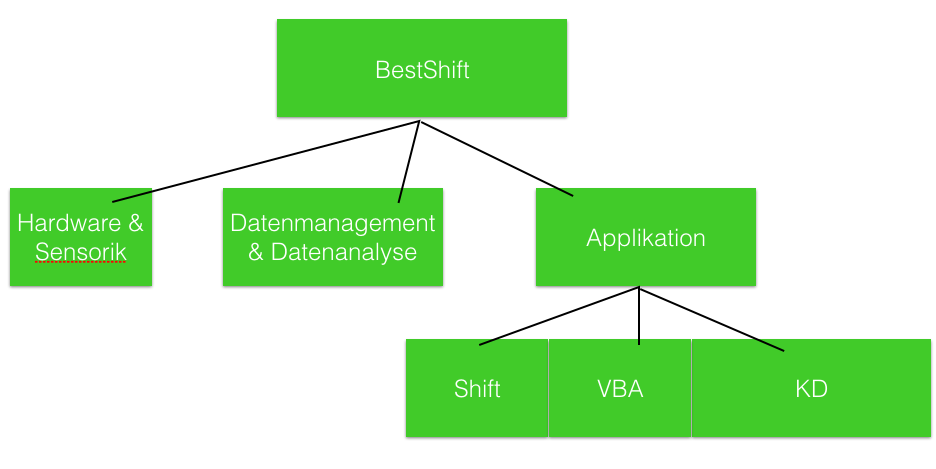
\includegraphics[scale=0.5]{images/Workflowdiagramm.png}

\newline
\section{Workflow des Projektes}
	\subsection{Tobias Perny - Hardware und Sensorik}
	Tobias Perny ist im Projekt wie bereits erwähnt für die Hardware und Sensorik zuständig. Er arbeitet mit einem Raspberry Pi2 Single Board Computer (SBC) auf welchem verschiedene Sensoren direkt montiert sind, welche dann interpretiert werden. Zusätzlich dazu ließt der Raspberry Pi2 die OBD-II Motordaten aus stellt diese zur Speicherung bereit.

	\subsection{Daniel Melichar - Datenmanagement und Datenanalyse}

	\subsection{Raphael Simsek - Schaltvorgangsvorschlag}

	\subsection{Hüseyin Bozkurt - Verbrauchsanalyse}

	\subsection{Fitim Faiku - Fahrkomfortanalyse}

>>>>>>> 44bfd702ec9a19dd5e03de0d417c2ea9aa7a82b6
